\documentclass{article}
\usepackage[utf8]{inputenc}
\usepackage[a4paper, total={7in, 9in}]{geometry}
\usepackage{amsmath, amssymb}
\usepackage{bm}
\usepackage{graphicx}
\usepackage{caption}
\usepackage[colorlinks=true]{hyperref}

\title{Transition path sampling and the calculation of free energies: trials and tribulations}
\author{Schwartz group}
\begin{document}
\maketitle
\section*{Probability distribution functions}

The probability distribution function for a point in the phase space ($\mathbf{x} = {\mathbf{r,p}}$) is given by 
\begin{equation}
P(\mathbf{x}) = \frac{e^{-\beta E(\mathbf{x})}}{\mathcal{Z}},
\end{equation}
where $\mathcal{Z}$ is the caninical partition function defined through the 
Hamiltonian of the system as 
\begin{equation}
\mathcal{Z} = \int e^{-\beta\hat{H}} d\mathbf{r}d\mathbf{p}.
\end{equation}

\section*{Sampling the order parameter with the TPS ensemble}
Window based TPS simulations speed up sampling of rare events along reaction coordinates
without the use of explicit constraining potentials as is done with non-Boltzmann sampling 
methods such as the umbrella sampling. Here, we briefly describe a procedure for practical calculation of the probability distribution function using an ensemble of TPS trajectories.

Consider an order parameter $\lambda(\mathbf{r})$ which is a reduced coordinate describing
the reaction of interest such that the definitions of the reactant state and the product 
state are easily stated. 
Furthermore, divide the order parameter into $n_w$ windows between the reactant and the product states and start $n_t$ trajectories within each window with a time step
of $\tau$ and a total number of frames of $n_{f}$ which results in a total time of $T = \tau\times n_f$ for each trajectory. Since there are no constraining potentials, trajectories which start in a window are free to evolve into other windows which is dictated only by the underlying free energy surface. Consider the probability of observing an order parameter interval defined as $\lambda_i$, given that we define the frequency of observing $\lambda_i$
in two different ways. 
%The first is considering only the sampled points for a particular window and the second is based on cumulative sampling which considers all the sampled trajectories across all the windows. 
\begin{align}
n_{\lambda_i} &= \sum_{j=1}^{n_f\times n_t} \delta(\lambda_j - \lambda_i) \label{nwin}\\
\tilde{n}_{\lambda_i} &= \sum_{j=1}^{n_w\times n_f\times n_t} \delta(\lambda_j - \lambda_i) \label{ntotwin}
\end{align}
where Eq. \ref{nwin} refers to the total number of times $\lambda_i$ is observed while 
only considering trajectories sampled wihtin a particular window and Eq. \ref{ntotwin}
refers to the total number of times $\lambda_i$ is observed over all trajectories across
all windows. To obtain an estimate of the probability distribution of $\lambda_i$, we need to divide this frequency with the total number of frames which results in

\begin{align}
P(\lambda_i) &= \frac{n_{\lambda_i}}{n_f\times n_t} \\
\tilde{P}(\lambda_i) &= \frac{\tilde{n}_{\lambda_i}}{n_f\times n_t\times n_w}
\end{align}

The potential of mean force for a given window with order parameter $\lambda_i$ can be obtained as 
\begin{equation}
F(\lambda_i) = -k_{B}T[ln(P(\lambda_i))] + C_i
\end{equation}
where $C_i$ is an undetermined constant which needs to be fixed to make the free energy curve continuous across the windows.  
\section*{Calculation details and results}
These results are based on calcuations involving $\sim 1000$ trajectories of 50 frames each and a time step of 1 femtosecond performed for each of the windows. 
\begin{figure}[ht]
  \centering
  \begin{minipage}[b]{0.45\linewidth}
    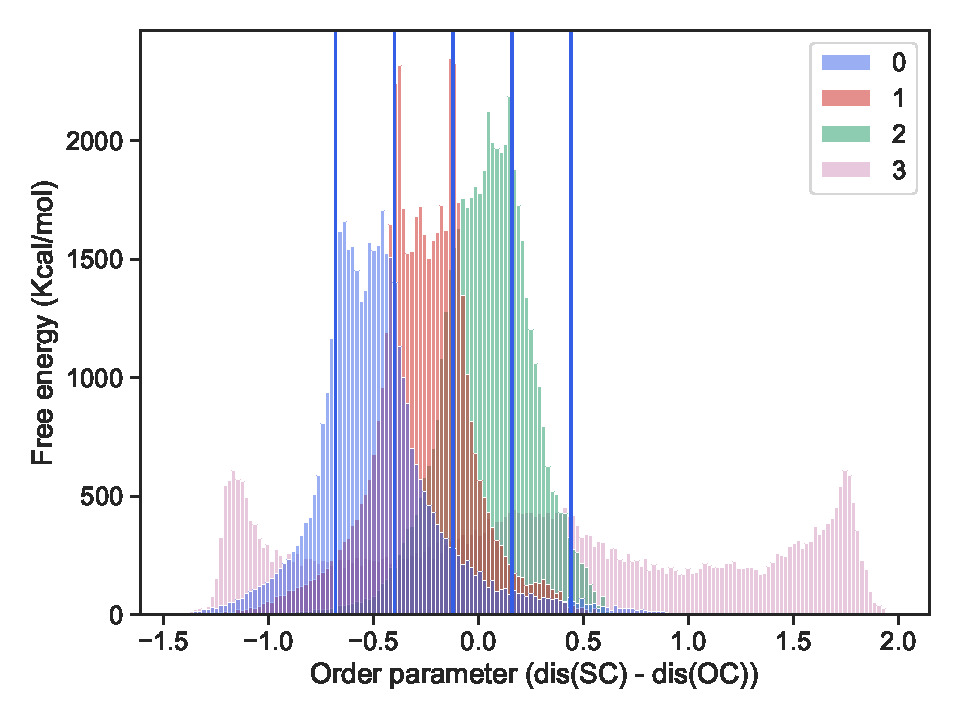
\includegraphics[scale=0.53]{figures/dist.pdf}
    %\caption{Distribution of the order parameter}
    \label{fig:dist}
  \end{minipage}
  \quad
  \begin{minipage}[b]{0.45\linewidth}
    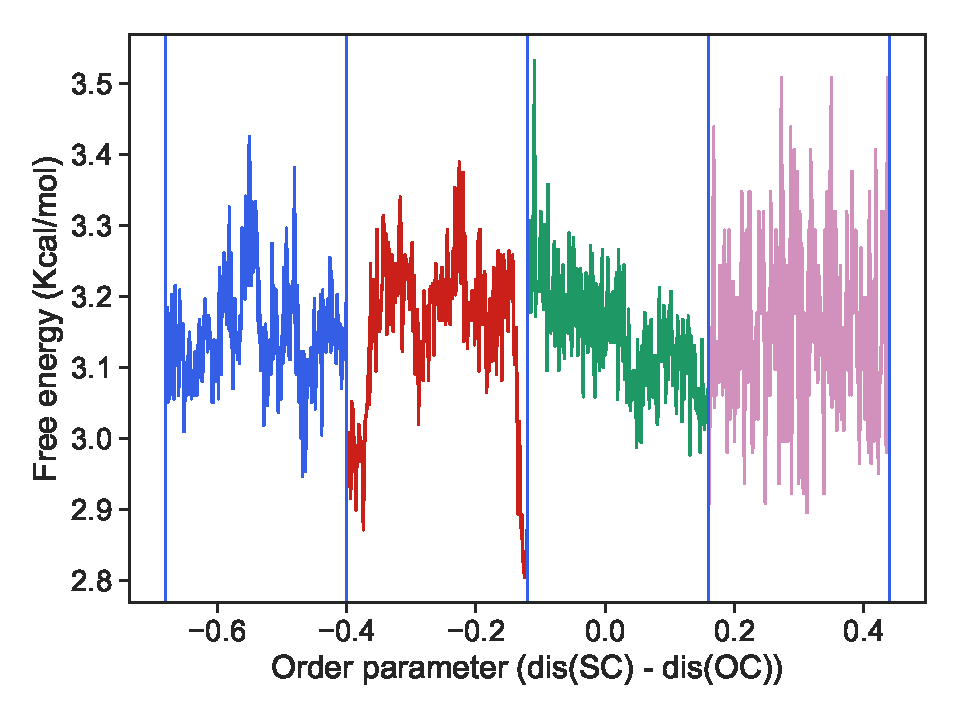
\includegraphics[scale=0.53]{figures/fenergy.pdf}
    %\caption{Free energy using Boltzmann inversion}
    \label{fig:fenergy}
  \end{minipage}
  \caption{The distribution of order parameters (left) considering only trajectories sampled wihtin a particular window and the corresponding free energy profile.}
\end{figure}

\begin{figure}[ht]
  \centering
  \begin{minipage}[b]{0.45\linewidth}
    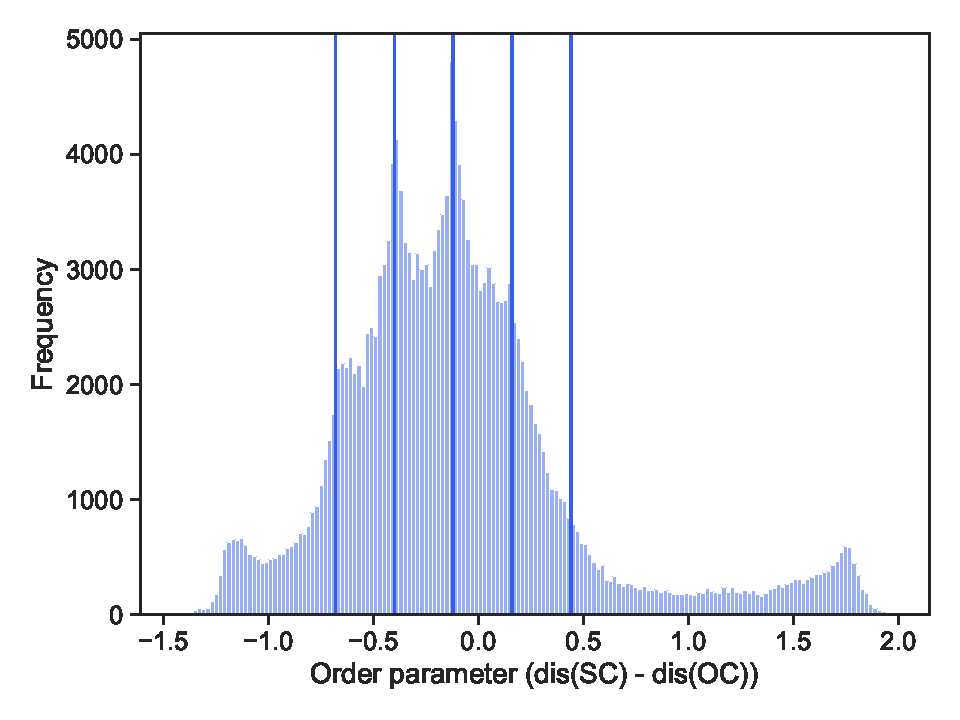
\includegraphics[scale=0.53]{figures/cumul-dist.pdf}
    %\caption{Cumulative distribution of $\bm{\lambda}$}
    \label{fig:cumdist}
  \end{minipage}
  \quad
  \begin{minipage}[b]{0.45\linewidth}
    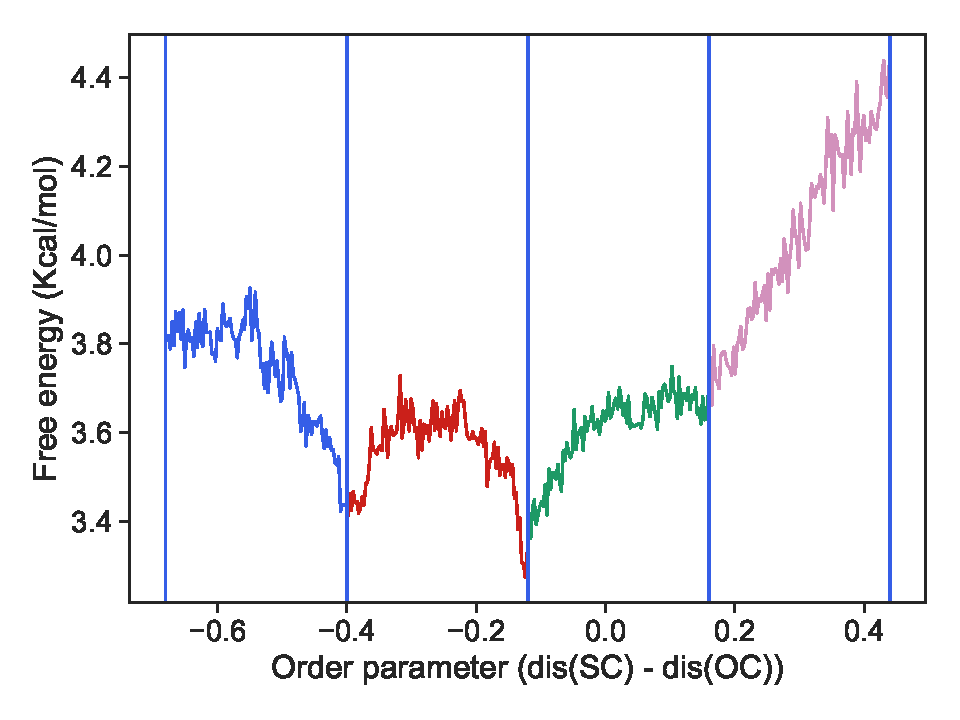
\includegraphics[scale=0.53]{figures/cumul-fenergy.pdf}
    %\caption{Free energy using Boltzmann inversion}
    \label{fig:cumfenergy}
  \end{minipage}
  \caption{The distribution of order parameters (left) considering all the sampled trajectories across all the windows and the corresponding free energy profile.}
\end{figure}
\end{document}
